\documentclass[12pt,a4paper]{article}
\usepackage[spanish,es-tabla]{babel}
\usepackage{bbm}
\usepackage[utf8]{inputenc}
\usepackage{multicol}
\usepackage[T1]{fontenc}
\usepackage{graphicx}
\usepackage{gensymb}
\usepackage{amssymb, amsmath} %Paquetes matemáticos de la American Mathematical Society
\parskip=1 mm
\oddsidemargin -0.8 cm
\headsep -2 cm
\textwidth=17.8cm
\textheight=25.5cm
\begin{document}
\title{Laboratorio de Mecanica, Practica 4 - Ley de Hooke}
\date{24 de febrero del 2025}
\author{\textbf{Ortega Montero Fernando Naed} - Equipo 4\\
Yibran Morales Munguía\\
Victor Manuel Santillan Romero}
\maketitle
\section{Resumen} 

Este informe de laboratorio tratara una practica de laboratorio donde se mide la elongación de un resorte de expansión usando diversas masas (y únicamente utilizando la fuerza de la gravedad) con el objetivo de encontrar la constante k del resorte y además una ecuación de la recta que describa la relación de la masa con la elongación. 

\section{Introducción}

La ley de Hooke es un principio físico que describe las deformaciones de un resorte provocadas por una fuerza ejercidas en su eje de simetría (el eje por el cual el resorte se comprime o expande de forma simétrica).  \\
La ley de Hooke enuncia que la fuerza aplicada sobre un resorte es directamente proporcional a su elongación por una constante, esto expresado matemáticamente sería…
\[F = -k \Delta x\]
Donde:\\

F : La fuerza ejercida sobre el resorte en su eje de simetría en newtons (N).\\

k : La constante del resorte, que mide la resistencia del resorte a las deformaciones, en newtons sobre metro ($\frac{N}{m}$).\\

$\Delta x$: La elongación del resorte; o la diferencia entre la longitud del resorte sin ninguna fuerza aplicada y la longitud del resorte bajo la existencia de una fuerza sobre él ($|x_ - x|  = \Delta x$), medida en metros (m).\\

Se puede notar que la constante k es negativa, esto se debe al carácter vectorial de la fuerza, donde indica que la dirección sobre la cual se aplica la fuerza es inversa a la dirección de la elongación. \\


\section{Desarrollo experimental}

Para esta práctica se utilizó un soporte universal, dos varillas con nuez, un resorte de expansión, una balanza granataria, flexómetro y un marco de pesas con gancho (Pesas de 50.0 g, 100.2 g, 200.3 g, 400.6 g, 500.2 g y 1000.0 g). \\

El resorte se colgó de una de las varillas en posición vertical, se midió la longitud del resorte con una masa 0, después se partió de una masa de 150.0 g con incrementos de 50 g, hasta llegar a los 600.0 g, se ahí se tomaron tres medidas mas una de 700.0 g una de 900.0 g y una última de 1000.0 g, en cada aumento de masa se midió la longitud del resorte con el flexómetro (Sin tomar en cuenta ni los aros que ayudan a colgar el resorte ni la longitud de los pesos colgados en el resorte) y la masa de las pesas (A pesar de que la balanza granataria no podía medir masas más allá de los 610.0 g, se asumió la masa de las últimas tres medidas por la indicación del fabricante).\\ 

Como no se tenían pesas en incrementos de 50.0 g se utilizaron combinaciones de las pesas nombradas anteriormente. \\

\section{Resultados}

En la tabla 1 se pueden apreciar las masas y elongaciones respectivas medidas durante el experimento, y en la Figura 1 se plasman estos resultados en una grafica.\\

\begin{table}[h]
\begin{center}
\begin{tabular}{|c|c|c|}
\hline
No. & Masa (g) & Elongación (cm) \\
\hline
0 & 0 & 20.0 cm \\
\hline
1 & 150.6 g & 21.1 cm\\
\hline
2 & 200.3 g & 23.2 cm\\
\hline
3 & 250 .7 g & 26.2 cm\\
\hline
4 & 300.9 g & 29.5 cm\\
\hline
5 & 350.9 g & 32.2 cm\\
\hline
6 & 400.7 g & 37.1 cm\\
\hline
7 & 450.9 g & 41.2 cm\\
\hline
8 & 500.1 g & 45.3 cm\\
\hline
9 & 551.2 g & 48.9 cm\\
\hline
10 & 601.2 g & 52.6 cm \\
\hline
11 & 700.0 g & 60.5 cm \\
\hline
12 & 900.0 g &  76.0 cm\\
\hline
13 & 1000.0 g & 83.7 cm\\
\hline
\end{tabular}
\caption{}
\end{center}
\end{table}

\begin{figure}[h!]
\centering
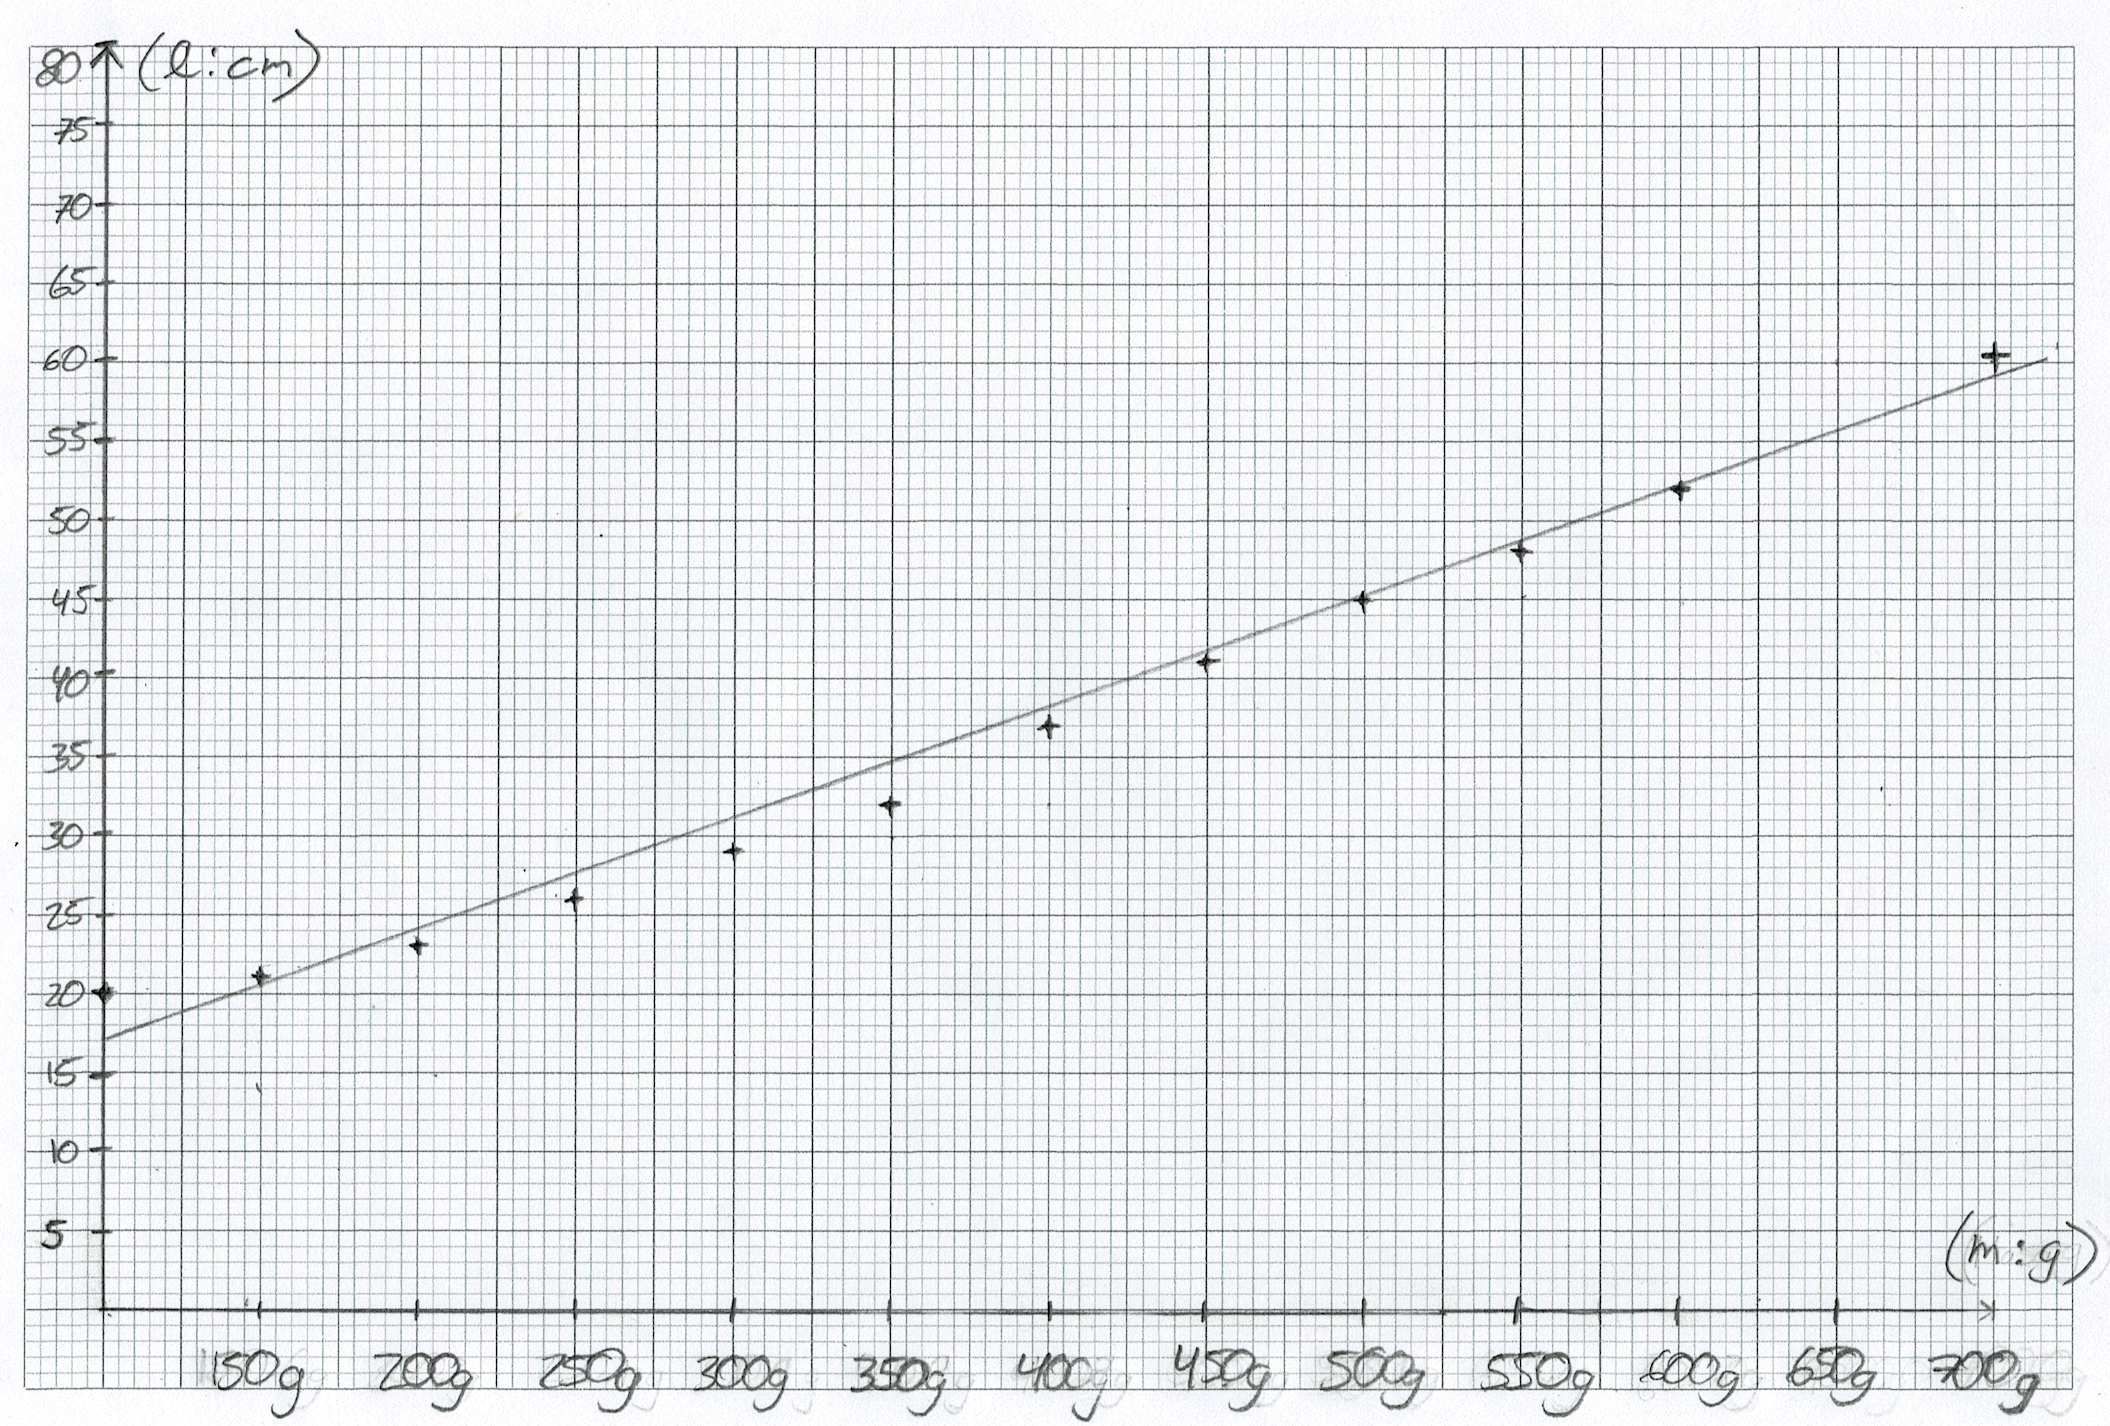
\includegraphics[scale=0.65]{1.png}
\caption{}
\end{figure}

\newpage


\section{Discusión}

Como se puede notar en la Figura 1 y en la Tabla 1, la incertidumbre estaría dada por la resolución del instrumento en ambos casos, donde la resolución del flexómetro es de 0.1 cm y la resolución de la balanza graduada es de 0.1 g, con esta información se hizo la aproximación lineal.\\
Con esta aproximación lineal se calculará la ecuación de la recta con la forma…
\[y = mx+c\]
Donde…\\
y = l, longitud en centímetros (cm).\\
x = m, masa en gramos (g).\\
m = k, constante del resorte en gramos sobre metro, para fines prácticos gramos sobre centímetro ($\frac{g}{cm}$)
c = $y_0$, la longitud del resorte en centímetros (cm).\\
Así obteniendo…
\[l = k m + y_0\]
Tomando dos puntos de la aproximación lineal, como se ve en la Figura 1, el $m_1 = 225 g$ con $l_1 = 26 cm$ y el punto $m_2 = 525 g$ con $l_2 = 47 cm$, con la fórmula de la pendiente $m = \frac{y_2 - y_1}{x_2 - x_1}$ y aplicando los cambios de notación antes mencionados tenemos…
\[k = \frac{l_2 -  l_1}{m_1 - m_2}\]
Así tenemos que k, en la aproximación lineal, es…
\[k = \frac{47 cm -  26 cm}{525 g - 225 g} = 0.07 \frac{cm}{g}\]
Y se puede notar también en la Figura 1 que $y_0 = 17 cm$, con esta información la ecuación de la recta ideal sería…
\[ l = 0.07 \frac{cm}{g} m + 17 cm\]
En este caso el error de la primera medición respecto de la recta ideal sería de 3 cm. 

\section{Conclusión}

La práctica fue llevada a cabo con éxito, como se enunció durante el desarrollo experimental las últimas tres masas no fueron medidas debido al limite de la balanza granataria, a pesar de esto fueron utilizadas por la curiosidad de ver el resorte expandirse mucho más y medir la elongación producida por masas grandes con relación a las masas anteriormente utilizadas. \\
Se realizó la practica con éxito bajo las indicaciones del profesor y además se lleno un poco nuestra curiosidad sobre estos fenómenos físicos.

\section{Referencias}

Martín, J. M. (2025) \textit{Física Experimental. Introducción a los conceptos y métodos.} Recuperado el 11, 02, 2025, de https://copitarxives.fisica.unam.mx/LT0006ES/LT0006ES.pdf \\

Alonso, V. (2018). Ley de Hooke.\\

Sanger, A. (2005). “LAS FUERZAS Y SU MEDICIÓN”: LEY DE HOOKE. Provincia de Santa Fe, Argentina: Malvinas Argentinas.\\

\end{document}